\section{Processi di Supporto}
I processi di supporto contribuiscono a rendere i processi primari più
efficienti ed efficaci.
\subsection{Documentazione}
\subsubsection{Descrizione}
Questa sezione contiene tutte le norme che ogni membro del gruppo dovrà seguire
durante la stesura della documentazione.\\ Fornisce le indicazioni utili per
ottenere una forma uniforme dei documenti e permette di operare seguendo linee
guida durante tutte le fasi del ciclo di vita di un documento: creazione,
stesura, verifica\textsubscript{g} ed eventuali modifiche, fino ad arrivare
all'approvazione\textsubscript{g} e quindi alla pubblicazione del documento.
\subsubsection{Ciclo di vita di un documento}
\begin{itemize}
    \item \textbf{Creazione}: viene creato un nuovo branch\textsubscript{g}, che prende il nome del documento stesso
          (vedi \nameref{inf:branch}) e in cui viene caricato il template. Dal momento della creazione, in questo
          branch\textsubscript{g} ci saranno solamente le versioni verificate del documento;
    \item \textbf{Stesura}: per la stesura verrà creato un sotto-branch\textsubscript{g}, caratterizzato dal numero della issue che richiede la stesura, in seguito si procede con la stesura delle sezioni necessarie, tracciando i cambiamenti nel registro delle modifiche e aggiornando la versione;
    \item \textbf{Verifica\textsubscript{g}}: prima di considerarsi completata, ogni modifica al documento deve essere verificata da un verificatore in carica, tramite una pull request\textsubscript{g} viene messo in esame quanto aggiunto al documento rispetto alla versione precedente, si presentano due casi:
          \begin{itemize}
              \item \textbf{Pull request\textsubscript{g} accettata}: il verificatore non trova errori e considera il lavoro 'verificato', quindi accetta la pull request\textsubscript{g} e fa il merge dal branch\textsubscript{g} di lavoro al branch\textsubscript{g} del documento, chiudendo la issue assegnata e il branch di lavoro;
              \item \textbf{Pull request\textsubscript{g} rifiutata}: il verificatore non considera la stesura adeguata e segnalare errori ed eventuali correzioni, la pull request\textsubscript{g} resta aperta e si continua a lavorare nel sotto-branch\textsubscript{g};
          \end{itemize}
    \item \textbf{Approvazione\textsubscript{g}}: Una volta che tutte le sezioni sono state verificate, e il documento è pronto per essere pubblicato, si procede con l'approvazione\textsubscript{g}, effettuata dal responsabile, utilizziamo questa procedura:
          \begin{itemize}
              \item Il verificatore che ha verificato l'ultima sezione completata apre una pull
                    request\textsubscript{g} per fare il merge dal branch\textsubscript{g} del
                    documento al main;
              \item Il responsabile rilegge ed analizza il documento nella sua interezza;
              \item Se riscontra errori o problematiche, segnala le modifiche necessarie e si
                    procede come descritto sopra;
              \item Nel caso di un verbale esterno, il responsabile genera il file '.pdf' e lo
                    invia al soggetto esterno con cui si è svolto l'incontro. Questi restituisce il
                    documento firmato. A questo punto il responsabile carica il verbale firmato
                    nella relativa cartella, e utilizza il comando \texttt{\char`\\includepdf} per
                    sostituire l'ultima pagina del verbale con quella firmata;
              \item Successivamente, aggiorna il registro delle modifiche aggiungendo una riga con la
                    versione di pubblicazione, e contrassegna il documento come 'Approvato';
              \item Infine, accetta la pull request e fa il merge dal
                    branch\textsubscript{g} del documento al main.
              \item Una Action di GitHub\textsubscript{g} si occupa di compilare il documento e di
                    renderlo disponibile pubblicamente in formato '.pdf'.
          \end{itemize}
\end{itemize}

\newpage
\subsubsection{Struttura}
Ogni documento è caratterizzato da un template, che presenta queste
caratteristiche:
\begin{itemize}
    \item \textbf{Intestazione}: la prima pagina di ogni documento, contiene:
          \begin{itemize}
              \item Logo del gruppo;
              \item Indirizzo email del gruppo;
              \item Titolo del documento;
              \item Informazioni sul documento, che comprendono:
                    \begin{itemize}
                        \item Versione;
                        \item Stato: in redazione oppure approvato;
                        \item Uso: interno o esterno;
                        \item Approvazione\textsubscript{g}: indica il nome dell'elemento del gruppo che ha
                              approvato il documento;
                        \item Redazione: indica il nome o i nomi di chi si è occupato della stesura;
                        \item Verifica\textsubscript{g}: indica il nome del verificatore o dei verificatori;
                        \item Distribuzione: elenco delle persone o organizzazioni a cui è destinato il
                              documento.
                    \end{itemize}
              \item Descrizione: una breve descrizione di cosa contiene il documento;
          \end{itemize}
    \item \textbf{Registro delle modifiche}: contiene la tabella dove verranno registrati i cambiamenti e le versioni che un documento attraversa prima di giungere alla versione finale, include le seguenti colonne:
          \begin{itemize}
              \item Versione;
              \item Data;
              \item Autore;
              \item Descrizione: una descrizione riassuntiva di ciò che è stato aggiunto o
                    modificato;
              \item Verificatore.
          \end{itemize}
    \item \textbf{Indice}: elenco ordinato dei titoli dei capitoli, per facilitare la navigazione;
    \item \textbf{Contenuto}: varia a seconda del documento.
\end{itemize}
% + tutte le convenzioni
\subsubsection{Convenzioni}
Al fine di ottenere una stesura della documentazione omogenea, e quindi più
professionale, verranno seguite queste convenzioni:
\paragraph{Date}
Per garantire un ordinamento in ordine cronologico in fase di pubblicazione,
dal più recente al meno recente, verrà utilizzato il formato
\textbf{yyyy-mm-dd} nel caso la data debba essere indicata nel nome del
documento (vale per verbali interni/esterni), per indicare una data all'interno
del documento, verrà utilizzato il formato \textbf{dd-mm-yyyy}.
\paragraph{Nomi di persona}
All'interno dei documenti i nomi di persona saranno rappresentati da cognome e
nome.
\paragraph{Elenchi puntati}
Gli elenchi puntati saranno gestiti in questo modo:
\begin{itemize}
    \item Ogni elemento dell'elenco deve iniziare con la lettera maiuscola;
    \item Ogni elemento dell'elenco deve terminare con ';', ad eccezione dell'ultimo che
          terminerà con '.';
    \item Dopo i due punti la prima parola deve iniziare con la lettera minuscola.
\end{itemize}
\paragraph{Stile del testo}
\begin{itemize}
    \item \textbf{Grassetto}: utilizzato per i titoli delle sezioni, per i sottotitoli, per i paragrafi e per parole tecniche o termini specifici che necessitano di evidenza nel contesto;
    \item \textbf{Corsivo}: utilizzato quando vengono scritti nomi di documenti, nome del gruppo o indirizzo email del gruppo.
\end{itemize}
\paragraph{Link}
All'interno dei documenti i link saranno strutturati in questo modo:
\begin{itemize}
    \item Breve descrizione della destinazione del link: \textbackslash
          url\{indirizzo\_del\_link\}.
\end{itemize}
\paragraph{Terminologia inglese}
Tutti i termini in lingua inglese saranno riportati al singolare, in quanto
questa scelta risulta più coerente con l'uso comune e l'assonanza nella lingua
italiana. Ad esempio, termini come "file" o "commit" verranno sempre utilizzati
nella loro forma singolare, anche quando si riferiscono a concetti plurali, per
evitare ambiguità o traduzioni non naturali.\\ Per quanto riguarda il genere
(maschile o femminile), verrà specificato all'interno del \textit{glossario},
così da uniformare l'interpretazione e garantire chiarezza, specialmente nei
casi in cui il termine inglese non abbia un corrispettivo diretto o il genere
non sia immediatamente evidente. Questa scelta mira a favorire una lettura
fluida e una comprensione condivisa del testo.
\paragraph{Acronimi}
Tutti gli acronimi seguiranno queste regole:
\begin{itemize}
    \item L'acronimo deve essere scritto in maiuscolo;
    \item L'articolo davanti a un acronimo deve concordare in genere e numero con il
          termine principale che l'acronimo rappresenta. Nel caso di acronimi derivati da
          termini stranieri, la concordanza va basata sul significato tradotto o
          percepito in italiano. Questo garantisce una corretta integrazione
          dell'acronimo nella struttura grammaticale della lingua;
    \item Ogni acronimo deve essere inserito nel glossario, accompagnato da una
          spiegazione dettagliata del suo significato, per garantire chiarezza e
          comprensione.
\end{itemize}
\subsubsection{Strumenti per la stesura}
Per la stesura dei documenti verrà usato il linguaggio LaTeX, un linguaggio di
marcatura per la preparazione di testi, basato sul programma di composizione
tipografica TEX, tutta la documentazione prodotta è contenuta nella cartella
'Docs'. I documenti seguono una struttura comune:
\begin{itemize}
    \item Cartella 'config' contenente il file 'changelog\_input' che permette di
          compilare i campi della tabella di registrazione delle modifiche;
    \item Cartella 'template' contenente:
          \begin{itemize}
              \item File 'changelog': questo file contiene la definizione di un comando chiamato
                    \texttt{\char`\\changelogTable}, che serve per generare la tabella formattata;
              \item File 'package': configura pacchetti e comandi per personalizzare
                    l'impaginazione, le tabelle, le intestazioni, la numerazione e la formattazione
                    di testo, inclusi glossari e codici;
              \item Cartella 'Images' contenente le immagini inserite nel documento.
          \end{itemize}
    \item File 'main' include i file e i pacchetti necessari a comporre il file;
    \item File 'titlepage' contenente il template della pagina di intestazione.
\end{itemize}
Oltre a questi files, verrà creato un file per ogni sezione, per garantire maggiore ordine all'organizzazione del documento, e facilitare la suddivisione dei compiti.
\subsubsection{Documentazione interna}
La documentazione interna è composta da tutti i documenti che contengono
informazioni utili per il gruppo, ma saranno comunque resi pubblici all'interno
del repository, e nella schermata creata tramite GitHub
Pages\textsubscript{g}.\\ La documentazione interna è composta da:
\begin{itemize}
    \item \textit{\textbf{Verbali Interni}}: hanno lo scopo di riportare ciò che viene detto e discusso durante la riunione interna, ossia tra i soli membri del gruppo,
          rispetta la struttura generale dei documenti e le convenzioni, il nome del file deve avere la forma 'VI\_yyyy-mm-dd', per garantire l'ordinamento.
          \\Nei \textit{verbali interni} la struttura del contenuto assume questa forma:
          \begin{itemize}
              \item \textbf{Informazioni generali}: contiene informazioni circa i dettagli sull'incontro, nello specifico:
                    \begin{itemize}
                        \item Luogo;
                        \item Data;
                        \item Ora di inizio;
                        \item Ora di fine;
                        \item Partecipanti.
                    \end{itemize}
              \item \textbf{Motivo della riunione}: breve descrizione narrativa di cosa è stato trattato in quell'incontro, descrive i motivi per cui è stata fatta la riunione;
              \item \textbf{Resoconto}: descrive i temi trattati nel dettaglio, partendo dal motivo per il quale sono stati sollevati e arrivando alla decisione presa dal gruppo a seguito di una discussione;
              \item \textbf{Prossimi obiettivi}: elenco puntato che descrive gli obiettivi che il gruppo si impegna a portare a termine nel breve periodo, indicativamente prima della riunione successiva;
              \item \textbf{Tracciamento delle decisioni}: tabella che riassume le decisioni prese in quella riunione indicandone:
                    \begin{itemize}
                        \item \textbf{Codice}: in formato VI Y.Z, dove Y indica il numero del \textit{verbale} (incrementale rispetto agli altri), Z indica il numero dell'argomento trattato (non per importanza, ma per ordine di discussione);
                        \item \textbf{Descrizione}: descrizione in poche parole dell'argomento trattato.
                    \end{itemize}
          \end{itemize}
    \item \textit{\textbf{Studio di fattibilità}}: documento interno di valutazione dei capitolati proposti dalle aziende per il progetto didattico, con lo scopo di selezionare il progetto migliore a cui candidarsi secondo valutazioni
          prese da parte del gruppo.\\
          Il documento, per ogni capitolato, espone una breve descrizione del prodotto che l'azienda chiede di sviluppare, seguito da una serie di pro e contro emersi in base a criteri soggettivi dei membri del gruppo.
          \\La valutazione è fatta sulla base di:
          \begin{itemize}
              \item \textbf{Presentazione del capitolato}: una presentazione più curata e dettagliata riscontra maggiore successo in fase di valutazione;
              \item \textbf{Interesse del gruppo al tema del progetto}: un capitolato porta con se un tema, viene valutato quanto ogni capitolato sia interessante, per apportare un impatto positivo allo svolgimento da parte del gruppo;
              \item \textbf{Tecnologie da utilizzare}: il contesto tecnologico di comune interesse porta maggiore produttività ed entusiasmo all'interno del gruppo;
              \item \textbf{Conoscenze pregresse}: un capitolato può risultare più o meno complicato da svolgere a seconda delle conoscenze acquisite nel percorso dai membri del gruppo;
              \item \textbf{Supporto da parte dell'azienda}: maggiore è il supporto offerto dall'azienda, migliore sarà la valutazione del capitolato.
          \end{itemize}
          Il documento offre una panoramica completa di tutti i capitolati, potendoli valutare minuziosamente prima di esprimere una valutazione.
    \item \textit{\textbf{Norme di progetto}}: documento interno che contiene le norme applicate dai membri del gruppo durante il ciclo di vita del prodotto, rispetta la struttura generale della documentazione, il corpo di questo documento è composto da:
          \begin{itemize}
              \item \textbf{Introduzione}: contiene una breve descrizione dello scopo del documento e del contesto in cui viene applicato;
              \item \textbf{Processi primari}: definizione dei processi primari, nel nostro caso:
                    \begin{itemize}
                        \item Fornitura: definizione e regole di fornitura e rapporto con il proponente;
                        \item Sviluppo: definizione e regole di sviluppo per quanto riguarda l'analisi dei
                              requisiti, la progettazione e la codifica.
                    \end{itemize}

              \item \textbf{Processi di supporto}: definizione dei processi di supporto, nel nostro caso:
                    \begin{itemize}
                        \item Documentazione: descrive le regole e la struttura dei documenti, il ciclo di
                              vita e le convenzioni da utilizzare durante la stesura. Vengono descritti i
                              documenti presenti nel repository;
                        \item Gestione della configurazione: descrive il versionamento dei documenti e la
                              struttura del repository;
                        \item Accertamento della qualità: descrive come vengono verificati i documenti;
                        \item Verifica: descrive come viene verificato il software;
                        \item Validazione: comprende le regole e la definizione di validazione.
                    \end{itemize}

              \item \textbf{Processi organizzativi}: costituisce la definizione dei processi per quanto riguarda l'organizzazione del gruppo, in termini di:
                    \begin{itemize}
                        \item Pianificazione: viene definito il metodo di lavoro, i ruoli che verranno
                              assegnati e le responsabilità che da essi ne derivano;
                        \item Modalità di comunicazione: vengono definite le modalità attraverso le quali il
                              gruppo comunicherà internamente ed esternamente (qualsiasi comunicazione che
                              comprenda un soggetto esterno al gruppo di lavoro);
                        \item Modalità di riunione: vengono definite le modalità con le quali si svolgeranno
                              le riunioni, interne ed esterne;
                        \item Gestione di infrastrutture: descrizione delle infrastrutture utilizzate per lo
                              sviluppo del progetto, affinchè venga garantita affidabilità e sicurezza;
                        \item Gestione dei dubbi o conflitti.
                    \end{itemize}

              \item \textbf{Standard di qualità ISO/IEC 9126}: descrizione dello standard scelto per garantire la qualità del software prodotto;
              \item \textbf{Standard di qualità ISO/IEC 12207:1995}: descrizione dello standard scelto per garantire la qualità dei processi relativi al ciclo di vita del software;
              \item \textbf{Metriche}: descrizione delle metriche adottate per la valutazione quantitativa dei processi e dei prodotti, spiegando in dettaglio
                    il significato di ogni metrica e il modo in cui le valutazioni vengono calcolate.

          \end{itemize}
\end{itemize}
\subsubsection{Documentazione esterna}
La documentazione esterna è composta da tutti i documenti che interessano anche
al proponente e al committente.
\begin{itemize}
    \item \textit{\textbf{Verbali esterni}}: verbali frutto di incontri fra i membri del gruppo e soggetti esterni ad esso.\\
          Seguono la struttura dei verbali interni, il nome del file deve avere la forma 'VE\_yyyy-mm-dd', cambia il processo di approvazione\textsubscript{g} del documento:
          il verbale viene approvato non solo dal responsabile, ma anche dal soggetto esterno con il quale si è svolto l'incontro,
          per rendere il documento più professionale e garantire coerenza tra il gruppo e il soggetto esterno.
    \item \textit{\textbf{Lettera di candidatura}}: la \textit{Lettera di candidatura} serve per esprimere la volontà di candidarsi allo svolgimento del capitolato scelto dopo aver discusso e redatto lo \textit{Studio di fattibilità},
          è composta da:
          \begin{itemize}
              \item Pagina iniziale: viene dichiarato il capitolato per il quale il gruppo ha
                    deciso di candidarsi, elencando i capitolati che più hanno riscontrato
                    interesse da parte del gruppo, inoltre espone una descrizione di cosa
                    aspettarsi dal contenuto del documento;
              \item Resoconto degli incontri: una breve descrizione degli incontri svolti con le
                    aziende riguardo i capitolati elencati nella pagina iniziale;
              \item Motivazione della scelta: espone il motivo per il quale il gruppo ha scelto il
                    capitolato a cui candidarsi.
          \end{itemize}
    \item \textit{\textbf{Diario di bordo}}: documento informale ad uso esterno che permette di interagire settimanalmente con il committente per riportare aggiornamenti sullo stato di
          avanzamento del progetto, descrivendo tutto ciò che è stato fatto rispetto al \textit{Diario di bordo} precedente,
          e quello che il gruppo si impegna a fare nel periodo successivo, vengono inoltre riportati dubbi e domande da porre al committente.
          Vengono elaborati tramite la piattaforma online 'Canva.com', che permette di creare presentazioni collaborative, accessibili online.\\
          La struttura del \textit{Diario di bordo} è composta da 4 slides contenenti:
          \begin{itemize}
              \item \textbf{Slide 1}: slide di presentazione che contiene:
                    \begin{itemize}
                        \item Logo;
                        \item Nome del gruppo;
                        \item Indirizzo email del guppo;
                        \item Titolo del documento: il titolo del \textit{Diario di bordo} segue una sintassi
                              prefissata ovvero 'Diario di bordo \#N', dove N è un numero che incrementa ad
                              ogni presentazione.
                    \end{itemize}
              \item \textbf{Slide 2}: contiene ciò che è stato svolto nel periodo trascorso;
              \item \textbf{Slide 3}: contiene ciò che il gruppo si impegna a portare a termine nel periodo successivo;
              \item \textbf{Slide 4}: contiene dubbi da chiarire e difficoltà incontrate dal gruppo.
          \end{itemize}
    \item \textit{\textbf{Piano di progetto}}: il documento \textit{Piano di progetto} ha lo scopo di supportare la gestione delle risorse per quanto riguarda l'avanzamento del progetto, per riuscire a portarlo a termine entro la data decisa.\\
          Il \textit{Piano di progetto} ha inoltre la funzione di descrivere il modello di sviluppo adottato, e di monitorarlo tramite la suddivisione in periodi, per analizzare il lavoro svolto e poter apportare miglioramenti con il passare del tempo.
          \\La struttura del documento segue la struttura generale, per quanto riguarda il corpo, è composto da queste sezioni:
          \begin{itemize}
              \item \textbf{Introduzione}: breve introduzione che descrive cosa aspettarsi dal contenuto del documento, sezione composta da:
                    \begin{itemize}
                        \item Scopo del documento;
                        \item Scopo del prodotto;
                        \item Riferimenti normativi e informativi.
                    \end{itemize}
              \item \textbf{Analisi dei rischi}: sezione che riassume i rischi a cui il gruppo si espone a seguito dell'aggiudicazione del capitolato, suddivisi in:
                    \begin{itemize}
                        \item Rischi riguardanti i requisiti;
                        \item Rischi tecnologici;
                        \item Rischi organizzativi;
                        \item Rischi personali.
                    \end{itemize}
              \item \textbf{Modello di sviluppo}: sezione che descrive il modello di sviluppo adottato dal gruppo, che si basa su un approccio agile. Viene fornita una descrizione completa del modello, illustrandone i principi fondamentali, le metodologie applicate e le motivazioni che hanno portato alla scelta di questo approccio;
              \item \textbf{Pianificazione}: sezione che descrive lo svolgimento delle attività suddiviso per periodi, fornendo un riassunto degli obiettivi previsti per ciascuno Sprint. Verranno indicati i risultati che il gruppo intende raggiungere e sarà incluso un diagramma di Gantt per visualizzare la pianificazione delle tempistiche e il progresso delle attività;
              \item \textbf{Preventivo}: sezione in cui viene pianificata in dettaglio la suddivisione dei ruoli con le corrispondenti ore di lavoro, per fornire un preventivo rispetto al periodo a cui ci si sta accingendo;
              \item \textbf{Consuntivo}: sezione che presenta i dati raccolti al termine di ciascun periodo, confrontandoli con le previsioni indicate nella sezione di preventivo. Verranno riportate le ore effettive di lavoro svolte e il relativo costo, accompagnati da un resoconto dettagliato che confronta le stime iniziali con i valori effettivi. Questo confronto permette di valutare eventuali scostamenti e di analizzarne le cause;
              \item \textbf{Attualizzazione dei rischi}: sezione dove vengono riportati i rischi che si sono verificati durante lo svolgimento del progetto e le relative misure di mitigazione attuate.
          \end{itemize}

    \item \textit{\textbf{Piano di qualifica}}: il documento \textit{Piano di qualifica} descrive i principi guida e le attività messe in atto dal team per assicurare che i processi adottati e prodotti sviluppati durante lo svolgimento del progetto siano di alta qualità per quanto riguarda le misure di efficienza ed efficacia.\\
          In questo documento verranno presentati i risultati delle analisi quantitative condotte per valutare le performance del team, evidenziando eventuali criticità e azioni correttive intraprese.
          \\La struttura del documento segue la struttura generale. Per quanto riguarda il corpo, è composto da queste sezioni:
          \begin{itemize}
              \item \textbf{Introduzione}: breve introduzione che descrive cosa aspettarsi dal contenuto del documento, riporta lo scopo del documento, lo scopo del prodotto, i riferimenti normativi e informativi;
              \item \textbf{Qualità di processo}: viene indicato lo standard adottato per la valutazione dei processi e quello per garantire un miglioramento continuo.\\
                    Seguono poi quattro sezioni:
                    \begin{itemize}
                        \item \textbf{Processi primari}: riporta una descrizione dei processi di fornitura e di sviluppo, e specifica le metriche per l'accertamento della qualità;
                        \item \textbf{Processi di supporto}: riporta una descrizione dei processi di documentazione, accertamento della qualità e verifica, specificando per ogni processo le metriche utilizzate;
                        \item \textbf{Processi organizzativi}: riporta una descrizione del processo di gestione di progetto e specifica le metriche da adottare per garantirne la qualità;
                        \item \textbf{Metriche}: contiene una tabella con le metriche adottate per la valutazione della qualità di processo, riportandone:
                              \begin{itemize}
                                  \item \textbf{Codice identificativo}: costituito da MPC[N], dove N rappresenta il numero della metrica di riferimento;
                                  \item \textbf{Nome}: nome della metrica;
                                  \item \textbf{Valore accettabile}: valore minimo accettabile per la metrica;
                                  \item \textbf{Valore ottimale}: valore ottimo per la metrica.
                              \end{itemize}
                    \end{itemize}
              \item \textbf{Qualità di prodotto}: viene indicato lo standard di riferimento adottato dal team per garantire la qualità del software e della documentazione prodotta.
                    \begin{itemize}
                        \item \textbf{Documenti}: riporta una descrizione dei parametri su cui si basa la valutazione della documentazione prodotta, ovvero comprensibilità e correttezza, e si riportano le metriche di riferimento;
                        \item \textbf{Software}: fornisce una descrizione degli obiettivi prefissati dal team per garantire la qualità nella produzione del software, focalizzandosi sui seguenti aspetti:
                              \begin{itemize}
                                  \item Funzionalità;
                                  \item Affidabilità;
                                  \item Usabilità;
                                  \item Efficienza;
                                  \item Manutenibilità;
                                  \item Portabilità.
                              \end{itemize}
                              Fornendone una descrizione e riportando le metriche di riferimento.
                        \item \textbf{Metriche}: contiene una tabella con le metriche adottate per la valutazione della qualità di prodotto, riportandone:
                              \begin{itemize}
                                  \item \textbf{Codice identificativo}: costituito da MPD[N], dove N rappresenta il numero della metrica di riferimento;
                                  \item \textbf{Nome}: nome della metrica;
                                  \item \textbf{Valore accettabile}: valore minimo accettabile per la metrica;
                                  \item \textbf{Valore ottimale}: valore ottimo per la metrica.
                              \end{itemize}
                    \end{itemize}
          \end{itemize}
    \item \textit{\textbf{Glossario}}: documento che contiene il significato dei termini chiave utilizzati nel progetto (indicati con il pedice 'g'), organizzati in ordine alfabetico, utile per garantire una comprensione comune fornendo spiegazioni concise e precise.
          \\La struttura del \textit{glossario} è composta da sezioni caratterizzate dalle lettere dell'alfabeto in ordine alfabetico, contenenti le parole che hanno come iniziale quella lettera.
\end{itemize}

\subsubsection{Metriche}
Per perseguire la qualità nel processo riguardo la documentazione si è deciso
di adottare le seguenti metriche:
\begin{itemize}
    \item \nameref{M:DOCC};
    \item \nameref{M:GI};
    \item \nameref{M:GE};
\end{itemize}

\subsection{Gestione della configurazione}
\subsubsection{Scopo}
La gestione della configurazione è un processo che mira a gestire e controllare
i cambiamenti apportati a un prodotto software o a un sistema durante il suo
ciclo di vita. La gestione della configurazione per la documentazione descrive
come vengono identificate, controllate, tracciate e gestite le versioni di un
documento.
\subsubsection{Versionamento}
Ogni versione del documento è identificata da un codice di versione nel formato
\textbf{Z.Y.X} dove:
\begin{itemize}
    \item \textbf{Z}: il documento è pronto per una delle revisioni, ovvero tutte le modifiche precedenti sono state approvate dal responsabile;
    \item \textbf{Y}: la sezione aggiunta o modificata di un documento è stata verificata;
    \item \textbf{X}: è stata corretta velocemente qualche incoerenza o errore minore.
\end{itemize}
\subsubsection{Repository}
Il repository si può trovare all'indirizzo
\textbf{\url{https://6bitbusters.github.io}} ed è pubblico. I collaboratori
sono i componenti del gruppo \textit{6BitBusters} che utilizzano il proprio
account GitHub personale per collaborare al progetto. La struttura del
repository è formata in questo modo:
\begin{itemize}
    \item \textbf{ .github}: cartella che contiene i file sorgenti delle GitHub Action e template per le issue;
    \item \textbf{3Dataviz}: cartella che contiene i file sorgente del prodotto;
    \item \textbf{Docs}: cartella che contiene la documentazione, si divide ulteriormente in:
          \begin{itemize}
              \item \textbf{Candidatura}: cartella che contiene i documenti da presentare per la candidatura;
              \item \textbf{Generali}: cartella che contiene tutta la documentazione esterna e interna tranne i verbali;
              \item \textbf{Verbali esterni}: cartella contenente i verbali esterni, che riportano gli incontri con i proponenti;
              \item \textbf{Verbali interni}: cartella contenente i verbali interni, relativi agli incontri tra membri del gruppo.
          \end{itemize}
    \item \textbf{website}: cartella che contiene i file sorgente del sito web che successivamente verrà pubblicato utilizzando GitHub Pages.
\end{itemize}
Infine il repository è dotato di sistema di auto-build per la documentazione grazie a GitHub Actions. Nello specifico sono stati scritti due tipi di Action
\begin{itemize}
    \item Per il push sul branch "main" che ha il compito di compilare tutta la
          documentazione creata fino a quel momento e di \textbf{creare la page};
    \item Per un test di compilazione solamente della parte aggiunta nel branch derivato,
          questo test deve essere \textbf{passato con successo} in modo da sbloccare
          l'azione di merge.
\end{itemize}
Per maggiori informazioni riguardanti i branch seguire le regole descritte nella sezione \nameref{inf:branch}

\subsubsection{Branching}\label{inf:branch}
I branch si dividono in:
\begin{itemize}
    \item \textbf{Branches protetti}:
          \begin{itemize}
              \item \textbf{main}: branch principale che contiene la documentazione e codice approvato del responsabile, non che la parte che viene mostrata sulla page;
              \item \textbf{docs/NOME-DOCUMENTO}: sono più branch che contengono solamente le versioni di documenti verificate;\\
                    Il nome di questi branch deve essere:
                    \begin{center}
                        \textbf{\textit{docs/[NOME-DOCUMENTO]}}
                    \end{center}
                    dove:
                    \begin{itemize}
                        \item \textbf{NOME-DOCUMENTO}: indica il nome del documento in questione.
                    \end{itemize}
          \end{itemize}
    \item \textbf{Branches derivati}: sono branch utilizzati per aggiungere modifiche e aggiornare un documento o una parte di codice che poi dovrà essere verificata
          attraverso una pull request verso il branch da cui esso è stato derivato;\\
          I nomi di questi branch, per quanto riguarda la documentazione, si suddividono in 2 casi:
          \begin{itemize}
              \item \textbf{Per Glossario}:
                    \begin{center}
                        \textbf{\textit{docs/glossario-[COGNOME-ASSEGNATARIO]}}
                    \end{center}
              \item \textbf{Per tutto il resto della documentazione}:
                    \begin{center}
                        \textbf{\textit{docs/[NOME-DOCUMENTO]-[ID-ISSUE]}}
                    \end{center}
          \end{itemize}
          dove:

          \begin{itemize}
              \item \textbf{NOME-DOCUMENTO}: indica il nome del documento sul quale si sta lavorando;
              \item \textbf{ID-ISSUE}: indica il numero identificativo associato alla issue relativa alla modifica del documento;
              \item \textbf{COGNOME-ASSEGNATARIO}: indica il cognome del membro che ha redatto il documento.
          \end{itemize}
          Nel caso un componente volesse richiedere una pull request ma il branch di destinazione fosse più aggiornato di quello di partenza o derivato, il branch protection
          impone che avvenga un merge dal branch di destinazione a quello di partenza in modo tale da applicare le modifiche delle versioni già approvate, al documento, che ne contiene
          altre e che di conseguenza deve passare ad una versione successiva.
    \item \textbf{Branch di hotfix}: sono branch dedicati all'hotfix e quindi a correzioni minime, sia per la documentazione che per il codice. Valgono le stesse regole dei
          branch protetti, quindi le modifiche devono essere sempre verificate e in caso approvate.
          Il nome per questi branch deve essere:
          \begin{center}
              \textbf{\textit{hotfix/[NOME-DOCUMENTO]}}
          \end{center}
          dove:

          \begin{itemize}
              \item \textbf{NOME-DOCUMENTO}: indica il nome del documento che viene modificato.
          \end{itemize}
\end{itemize}

In ogni branch secondario il lavoro può essere svolto da un solo componente del
gruppo, specificatamente colui che ha preso in carico l'issue alla cui
risoluzione quel branch è dedicato.

Una volta che la issue viene risolta il componente deve richiedere una pull
request verso il branch da cui esso è stato derivato. Notare che se il branch
di destinazione è:
\begin{itemize}
    \item \textbf{main} $\rightarrow$ il documento deve essere approvato;
    \item \textbf{docs/NOME-DOCUMENTO} $\rightarrow$ il documento deve essere verificato e successivamente viene eliminato il branch derivato.
\end{itemize}

Di seguito si riporta un semplice ma esaustivo esempio di workflow tramite
immagine:
\begin{center}
    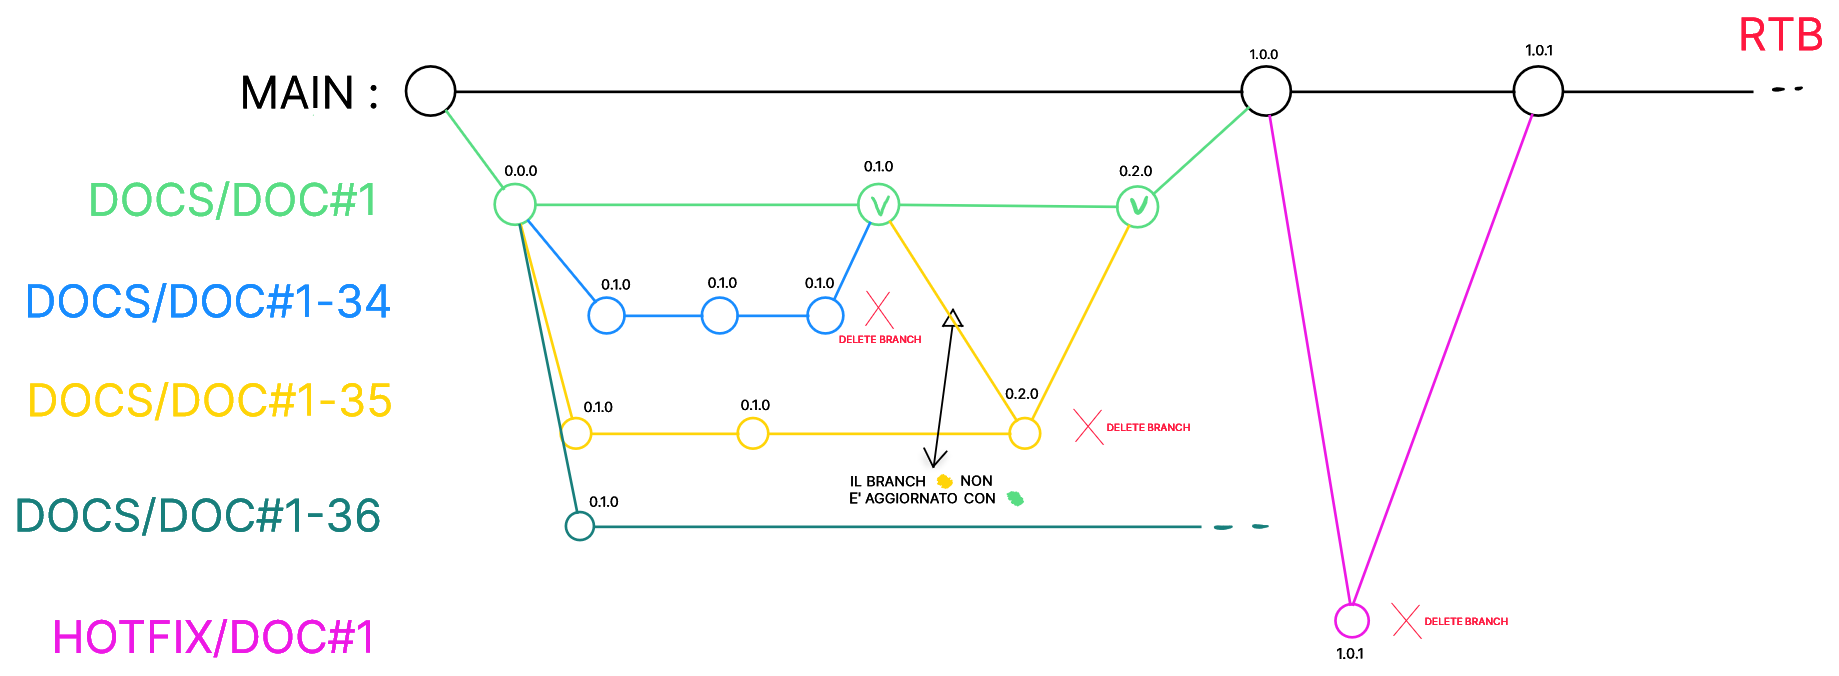
\includegraphics[scale = 0.33]{template/images/workflow.png}
\end{center}

\subsubsection{Commit}\label{inf:comm}
È preferibile che ogni commit abbia una singola responsabilità per cambiamento.
I commit non possono essere effettuati direttamente sui branch protetti ma per contribuire con delle aggiunte o
modifiche sarà necessario aprire una pull request, motivo per il quale abbiamo introdotto dei branch derivati.
I messaggi di commit dovranno seguire la seguenti strutture sintattiche:
\begin{center}
    \textbf{add: [COSA]\\
    change: [COSA]\\
    restructure: [COSA]}
\end{center}
dove:
\begin{itemize}
    \item \textbf{add}: viene utilizzato quando si va ad aggiungere una nuova sezione/sottosezione ad un documento;
    \item \textbf{change}: viene utilizzato quando si va a modificare una o più sezioni/sottosezioni di un documento;
    \item \textbf{restructure}: indica una ristrutturazione del branch main per quanto riguarda l'organizzazione delle cartelle e/o la modifica di action o template di issue;
    \item \textbf{COSA}: breve descrizione di cosa di è aggiunto e/o fatto.
\end{itemize}

Notare però che dopo l'approvazione di una pull request tutti i commit relativi
verranno raggruppati in un unico commit, il cui titolo deve rispettare la
struttura sintattica descritta in seguito.
\begin{center}
    \textbf{Update: [NOME-DOCUMENTO]-[VERSIONE]}
\end{center}
dove:

\begin{itemize}
    \item \textbf{NOME-DOCUMENTO}: indica il nome del documento nel quale sono state verificate le modifiche;
    \item \textbf{VERSIONE}: indica il numero di versione aggiornata.
\end{itemize}
Per quanto riguarda il commento facoltativo, si lascia quello di default proposto da GitHub,
ovvero un elenco puntato di tutti i commit che verranno raggruppati.\\

Per aggiornare direttamente il main si è deciso di disabilitare temporaneamente
il protection, eseguire un commit con delle modifiche, con la struttura
sintattica elencata sopra, e in fine attivare nuovamente il protection. Questa
soluzione è stata adottata perché il team ritiene sia più veloce e semplice
apportare modifiche a template e action in questo modo rispetto che alla
creazione di un branch e ad un successivo pull request, inoltre il branch main
una volta ultimate le automazioni non verrà più modificato se non dai merge
scatenati dalle pull request.

\subsubsection{Pull request}\label{inf:pr}
Per effettuare un merge su un branch protetto si deve aprire, da GitHub, una
pull request. Questa permette di verificare il lavoro svolto prima di
integrarlo con un branch protetto ed eseguire un veloce test di compilazione
della sezione aggiunta. Alla creazione di una pull request bisogna associare:
\begin{itemize}
    \item \textbf{Title}: [NOME-DOCUMENTO]-[ID-ISSUE];
    \item \textbf{Verificatori in carica}: coloro che hanno il compito di trovare eventuali errori o mancanze e fornire un feedback
          riguardante il contenuto direttamente su GitHub attraverso un commento, sulla stessa pull request.
          Non sarà possibile effettuare il merge finché tutti i commenti di revisione non saranno stati risolti
          con, al termine, l'approvazione di almeno uno dei verificatori e il test di build non dia esito positivo;
    \item \textbf{Descrizione}: contiene una lista riassuntiva di ciò che è stato fatto includendo le issue completate, e quindi da chiudere,
          con la sintassi
          \begin{center}
              \textbf{\textit{close ID-ISSUE}}
          \end{center}
          in modo tale che vengano tutte chiuse in automatico quando la pull request verrà accettata;
    \item \textbf{Gli assegnatari}: coloro che hanno anche il compito di apportare le modifiche necessarie al documento;
    \item \textbf{Label}: riassume di che natura è la pull request.
\end{itemize}
dove:

\begin{itemize}
    \item \textbf{NOME-DOCUMENTO}: indica il nome del documento sul quale si sta lavorando e richiedendo l'approvazione;
    \item \textbf{ID-ISSUE}: indica il numero identificativo associato alla issue relativa alla modifica del documento.
\end{itemize}

Per una descrizione più dettagliata delle issue si faccia riferimento a
\nameref{inf:its}

Per i commit relativi alle pull request seguire le regole descritte nella
sezione \nameref{inf:pr}

\subsection{Automazione}
\subsubsection{Scopo}
Lo scopo dell'automazione è garantire una maggiore efficienza e ridurre il
rischio di errori umani. Tuttavia, il costo necessario per rendere automatiche
alcune attività potrebbe essere superiore al beneficio ottenuto. È quindi
fondamentale scegliere attentamente quali processi automatizzare.
\subsubsection{Automazioni realizzate}
L'automazione dei processi di verifica e di compilazione della documentazione
avviene tramite GitHub Actions, che permette di eseguire script personalizzati
in risposta a eventi specifici che si verificano nel repository. In
particolare, sono state scritte tre diverse Action:
\begin{itemize}
    \item \texttt{build.yml}: si scatena a seguito di un push sul main; ha il compito di compilare
          tutta la documentazione creata fino a quel momento e di creare la relativa pagina web tramite Pages;
    \item \texttt{pr\_build\_check.yml}: si scatena quando viene effettuata una pull request verso il main o verso
          un branch di documentazione, ovvero del tipo docs/[NOME-DOCUMENTO]. Serve per verificare che
          i sorgenti LaTeX compilino correttamente e che sia stato modificato uno e un solo documento;
    \item \texttt{pr\_gulpease\_check.yml}: si scatena quando viene effettuata una pull request verso il main o verso
          un branch di documentazione, ovvero del tipo docs/[NOME-DOCUMENTO]. Essa verifica che
          l'indice Gulpease del documento, espresso come media degli indici delle sezioni, sia maggiore o uguale a 50.
\end{itemize}
Per garantire la qualità dei documenti prodotti, è necessario che le Action \texttt{pr\_build\_check.yml}
e \\\texttt{pr\_gulpease\_check.yml} diano esito positivo. A tale scopo, è stato configurato il repository in modo
che non sia possibile effettuare il merge di una pull request se non sono soddisfatti entrambi i controlli.
Inoltre, per accelerare il processo di verifica, è fortemente raccomandato eseguire localmente gli script di test,
in modo da individuare e correggere eventuali errori prima di effettuare la pull request.
\subsubsection{Aggiungere un'Action}
Per aggiungere un'Action, è necessario seguire i seguenti passaggi:
\begin{itemize}
    \item Creare un file in linguaggio YAML nella cartella \texttt{.github/workflows} del
          repository, in cui si specificano i dettagli dell'Action. In particolare, è
          necessario definirne:
          \begin{itemize}
              \item Nome;
              \item Evento che la scatena;
              \item Job da eseguire;
              \item Azioni da compiere all'interno di ciascun job.
          \end{itemize}
    \item Se necessario al funzionamento dell'automazione, produrre uno o più script e
          inserirli nella cartella \texttt{.github}. Il linguaggio utilizzato per
          scrivere tali script è python, scelto per la sua comprensibilità e facilità di
          utilizzo;
    \item Disabilitare temporaneamente il protection del main;
    \item Effettuare un commit con le modifiche apportate (vedi \nameref{inf:comm});
    \item Riabilitare il protection del main.
\end{itemize}

\subsection{Accertamento della qualità}
\subsubsection{Scopo}
Lo scopo del processo di accertamento della qualità è garantire la qualità dei
processi adottati e del software prodotto, al fine di soddisfare le aspettative
degli stakeholder e i requisiti del progetto. Ciò avviene tramite le attività
di pianificazione della qualità, il controllo della qualita e il miglioramento
continuo.
\subsubsection{Descrizione}
Il piano della qualità comprende gli obiettivi di qualità che il team si
impegna a raggiungere e le metriche utilizzate per misurare il raggiungimento
di tali obiettivi. \\ Il controllo della qualità consite nella misurazione e
analisi degli indicatori di interesse, valutando il grado di raggiungimento
degli obiettivi di qualità. \\ Il documento \textit{Piano di qualifica} tratta
nel dettaglio le attività di pianificazione e controllo della qualità. \\
\subsubsection{Ciclo di Deming}
Per quanto riguarda l'attività di miglioramento continuo dei processi, il
gruppo adotta il ciclo di Deming. Si tratta di un metodo di gestione iterativo
che prevede quattro fasi:
\begin{itemize}
    \item \textbf{Plan}: pianificazione degli obiettivi e dei processi necessari per fornire
          risultati in accordo con i risultati attesi, attraverso la creazione di attese di
          produzione, di completezza e accuratezza delle specifiche scelte;
    \item \textbf{Do}: attuazione del piano, tramite l'esecuzione dei processi,
          lo sviluppo dei prodotti e la misurazione dei risultati ottenuti;
    \item \textbf{Check}: analisi e studio dei dati raccolti nella fase Do.
          I grafici possono rendere più facile il confronto tra risultati ottenuti e attesi;
    \item \textbf{Act}: consolidamento delle soluzioni che hanno dato buoni risultati e
          adozione di strategie correttive per migliorare ciò che non ha soddisfatto le aspettative,
          dopo averne compreso a fondo le cause. In questo modo, ogni iterazione del ciclo di Deming
          contribuisce ad aggiungere valore al processo.
\end{itemize}
\subsubsection{Metriche}
Per perseguire la qualità nel processo di accertamento di qualità si è deciso
di adottare le seguenti metriche:
\begin{itemize}
    \item \nameref{M:MM};
\end{itemize}
\subsection{Verifica}
\subsubsection{Scopo}
Lo scopo del processo di verifica\textsubscript{g} è quello di accertare che
non siano stati commessi errori nello svolgimento delle attività prefissate.
Questo processo viene applicato costantemente sia durante la stesura della
documentazione, che durante lo sviluppo del software.
\subsubsection{Descrizione}
La verifica verrà fatta in maniera efficace adottando questi metodi:
\begin{itemize}
    \item \textbf{Analisi statica}: non richiede esecuzione dell'oggetto di verifica, quindi applicabile a documentazione e codice, usata per accertare conformità e regole nonché assenza di difetti, adotteremo i due seguenti metodi di lettura:
          \begin{itemize}
              \item \textbf{Walkthrough}: processo in cui il team esamina documenti o codice, in modo strutturato ma informale. L'obiettivo è identificare errori, migliorare la qualità e favorire la comprensione;
              \item \textbf{Inspection}: processo di revisione più formale, in cui i veroficatori controllano documenti o codice per trovare errori e migliorare la qualità eseguendo una lettura mirata dell'oggetto di verifica. Segue regole precise e prevede momenti organizzati, come pianificazione, definizione lista di controllo, lettura e correzione dei difetti.
          \end{itemize}
    \item \textbf{Analisi dinamica}: richiede esecuzione dell'oggetto di verifica, quindi applicabile solo al codice, usata per accertare che il codice sia corretto, non introduca errori nel sistema e soddisfi i requisiti preposti.
\end{itemize}
\subsubsection{Verifica della documentazione} Al momento della necessità di modificare o aggiungere qualcosa a una sezione di
un documento, si procederà in questo modo:
\begin{enumerate}
    \item Verrà creata una issue che specifica l'attività di modifica o aggiunta da
          svolgere;
    \item Verrà creato un sotto-branch\textsubscript{g} chiamato
          'docs/\textit{nome\_del\_documento}-N' dove con N si intende il numero della
          issue di riferimento;
    \item Rimanendo in questo sotto-branch\textsubscript{g}, verrà aggiornato il
          documento;
    \item Una volta terminato, per iniziare il processo di verifica\textsubscript{g}
          verrà aperta una pull request\textsubscript{g};
    \item Uno tra i verificatori in carica durante quello sprint si assegnerà la verifica
          del documento e modificherà il registro delle modifiche compilando il campo
          'Verificatore';
    \item Se la pull request\textsubscript{g} avrà esito positivo, ci sarà il merge tra
          il sotto-branch\textsubscript{g} e il branch\textsubscript{g} principale del
          documento, con conseguente chiusura della issue e del sotto-branch;
    \item In caso di esito negativo, verranno segnalati gli errori da parte del
          verificatore tramite commenti, e il redattore si occuperà di risolverli
          continuando a lavorare nel sotto-branch\textsubscript{g}, fino ad avere il
          documento verificato.
\end{enumerate}

\subsubsection{Verifica del codice}
Il processo di verifica del codice si attua principalmente attraverso lo
sviluppo e l'esecuzione di test, che permettono di eseguire un'analisi dinamica
del software, ossia un'analisi che si concentra sul comportamento del programma
durante l'esecuzione. I test vengono progettati per garantire che il codice
funzioni correttamente in vari scenari e che rispetti i requisiti prefissati. I
principali tipi di test utilizzati in questo processo sono:
\begin{itemize}
    \item \textbf{Test di unità}: verificano il corretto funzionamento delle singole unità o funzioni del codice, testando piccoli blocchi di logica isolati. Questi test sono fondamentali per individuare errori precoci e garantire che ogni componente funzioni come previsto. Vengono scritti dal programmatore che implementa il modulo;
    \item \textbf{Test di integrazione}: verificano che i vari moduli o componenti del sistema interagiscano correttamente tra loro. Questi test sono particolarmente utili per identificare problemi che si verificano quando le diverse parti del sistema vengono messe insieme;
    \item \textbf{Test di regressione}: vengono eseguiti per verificare che le modifiche recenti al codice non abbiano introdotto nuovi errori o causato il malfunzionamento di funzionalità precedentemente funzionanti. Questi test sono essenziali per mantenere l'integrità del software durante lo sviluppo continuo;
    \item \textbf{Test di sistema}: testano il comportamento complessivo dell'applicazione in un ambiente che simula il più possibile l'ambiente di produzione. Questi test verificano che l'intero sistema funzioni come previsto sotto condizioni realistiche e che tutte le componenti siano correttamente integrate.
\end{itemize}
I test vengono identificati attraverso un codice con questa struttura:
\textbf{
    \[
        T[\text{Tipo}][ \text{N}]
    \]
}
\\Dove N è il codice del test ed è un valore univoco e il tipo può essere:
\begin{itemize}
    \item \textbf{U}: test di unità;
    \item \textbf{I}: test di integrazione;
    \item \textbf{R}: test di regressione;
    \item \textbf{S}: test di sistema.
\end{itemize}

\paragraph{Metriche}
Per perseguire la qualità nel processo di verifica di qualità si è deciso di
adottare le seguenti metriche:
\begin{itemize}
    \item \nameref{M:COC};
    \item \nameref{M:SC};
    \item \nameref{M:BC};
    \item \nameref{M:PTC};
    \item \nameref{M:LT};
    \item \nameref{M:ART};
    \item \nameref{M:CYC};
    \item \nameref{M:PPM};
    \item \nameref{M:LPM};
    \item \nameref{M:LPF};
    \item \nameref{M:CD};
\end{itemize}
\subsection{Validazione}
\subsubsection{Scopo}
Per la documentazione la validazione corrisponde alla pubblicazione del
documento nel branch\textsubscript{g} main.\\ Questo processo avviene dopo
l'ultima verifica\textsubscript{g} e sarà il responsabile a stabilire se il
prodotto è accettabile o ha bisogno di ulteriori verifiche.
